\chapter{CLOUDY AS A SUBROUTINE}
% !TEX root = hazy2.tex

\section{Overview}

\Cloudy\ is designed to be used as a subroutine of other, much larger,
codes.  When used this way a series of subroutine calls, described next,
are used to initialize the code, specify the initial conditions, do the
simulation, and finally examine the predictions.

A common strategy is to call the code to compute line intensities for
a large matrix of parameters.
The results of one such calculation is shown
in Figure \ref{fig:CIV_EW} (\citealp{Baldwin1995};
\citealp{Ferland2003}).
Such grids can be computed
in a few dozen hours on modern workstations, and offer far greater insight
to physical effects of changing model parameters than does a single model.

\begin{figure}
\centering
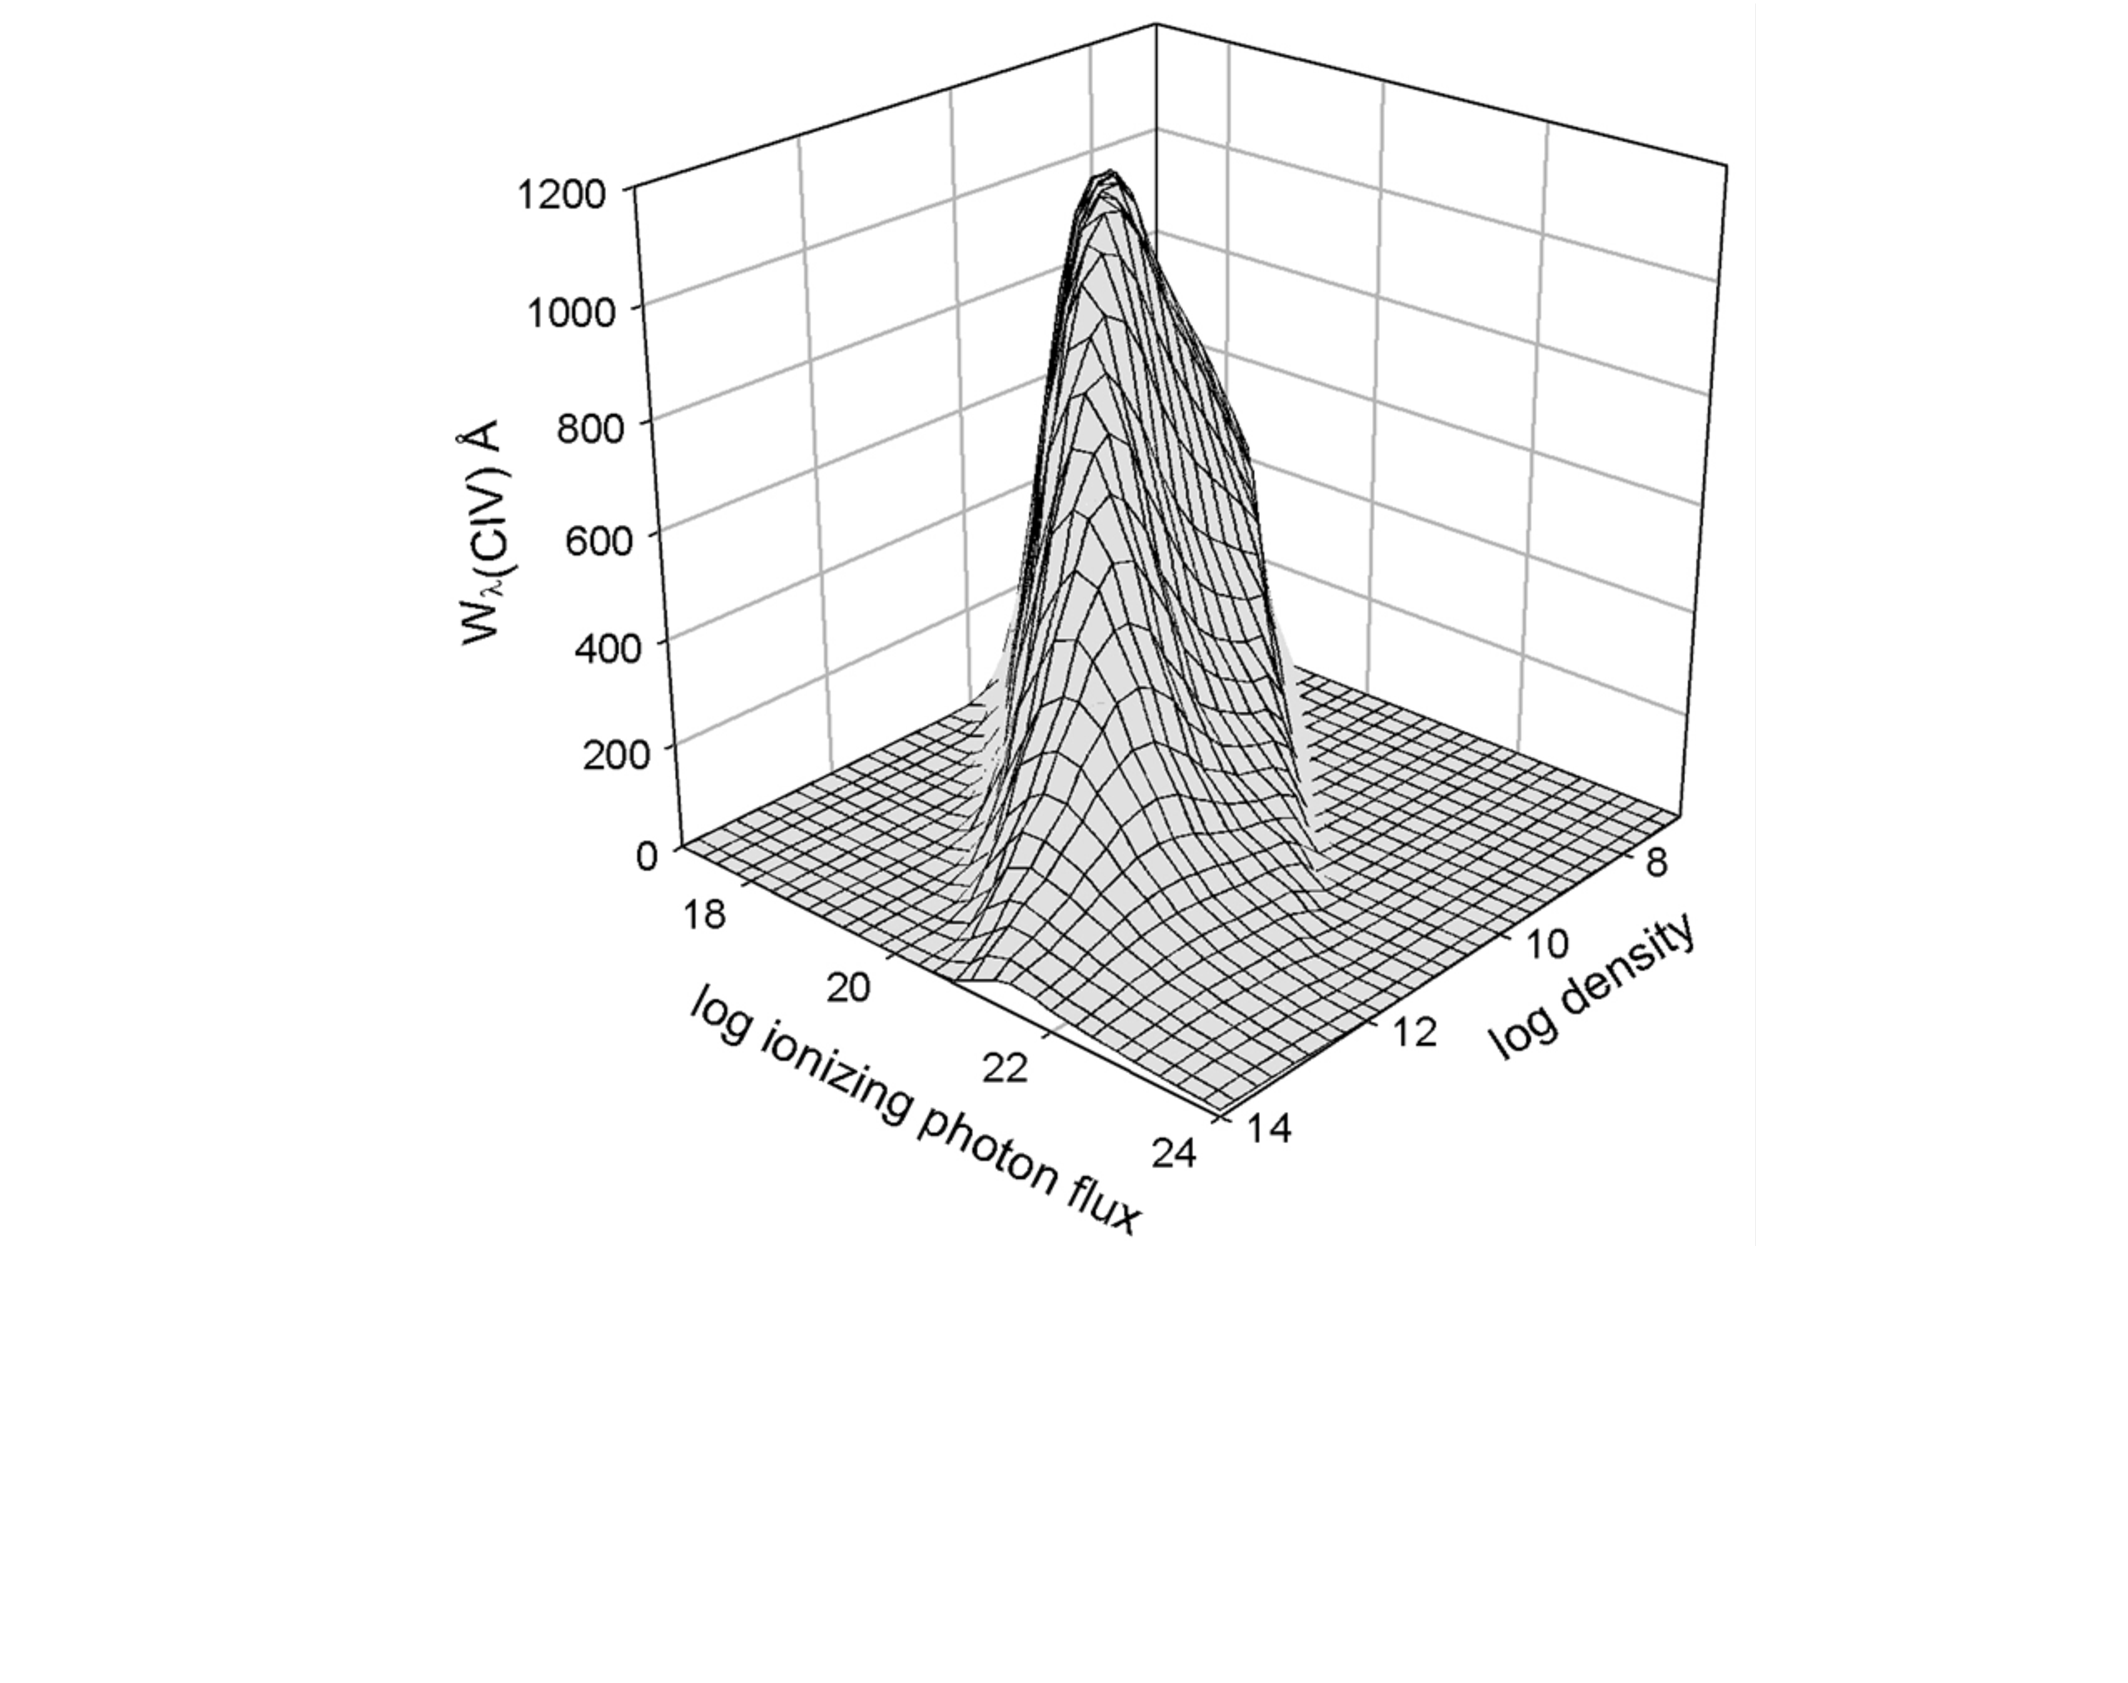
\includegraphics[scale=0.6]{CIV_EW}
\caption[C~IV equivalent width]{\label{fig:CIV_EW}The results of a large grid of quasar emission-line cloud
calculations are shown.  The $x$-$y$ plane shows the logs of the hydrogen density
(cm$^{3)}$ and flux of ionizing photons (cm$^{-2}$ s$^{-1}$).  The $z$ axis is the predicted
line equivalent width.}
\end{figure}

Much of this can be done without writing a program,
by using the \cdCommand{grid} command.
This command was introduced by Ryan Porter in C07.02, and makes
it possible to create large grids of models like those shown in
Figure \ref{fig:CIV_EW} with commands.
The \cdCommand{grid} command is described in Part 1 of this document.
There are several \cdCommand{save} output commands that are designed to save information
from grid calculations.

\begin{shaded}
\subsection{\experimental Host languages}

\Cloudy\ is written in C++, and it assumed for most of this section
that \Cloudy\ will be called from an external C or C++ program.

However, there is experimental support for a number of other
languages.

You can call a C++ program like \Cloudy\ from a Fortran program by
using the \cdTerm{cfortran.h} header file described at
\href{http://www-zeus.desy.de/~burow/cfortran/}{\tt
http://www-zeus.desy.de/$\sim{}$burow/cfortran/}.  I have never tried
this.  Good luck.

In the subdirectory \verb|sys_gcc_shared|, an additional set of
Makefile targets are set up to use the subroutine API described below
for Perl and Python scripts, using the SWIG interface generator.  In
this directory, there is also an experimental direct interface to the
Lua scripting language.
\end{shaded}

\subsection{Creating a new main program}

In C++ there must be exactly one main program
and it must be called \cdRoutine{main}.
This routine is within the file \cdFilename{maincl.cpp} in the source downloaded from
the web.
You need to replace the existing \Cloudy\ main program with one
that you write.
The file \cdFilename{maincl.cpp} that is included in the distribution
must be deleted so that the program you write will be loaded instead.
The
remaining routines are then compiled with a command like the following:
\begin{verbatim}
g++ -O3 -c *.cpp
\end{verbatim}
which will create a large number of object files.  The new main
program will then need to be linked with these object files with a
command something like
\begin{verbatim}
g++ -O3 -o mycloudy.exe newmain.cpp *.o -lm
\end{verbatim}

Alternatively, if you are using the Makefile build process and have
already built \Cloudy, you can use the library file \verb|libcloudy.a|
which contains all the object files with the command
\begin{verbatim}
g++ -O3 -o mycloudy.exe newmain.cpp -L. -lcloudy -lm
\end{verbatim}

The following subsections outline how to write code for this new main program.

\subsection{The cddefines.h and cddrive.h header files}

The file \cdFilename{cddrive.h} contains definitions of all public routines, the
routines that a user would call to drive \Cloudy.
That file is the definitive
reference for the material contained in this section and is more up to date
than this document.
Comments within that file explain all routines and
their parameters.

The header \cdFilename{cddefines.h} should come before \cdFilename{cddrive.h} since it includes
many definitions and includes the standard C++ header files that are needed
to drive the code.
The first two header files in the new main routine should
be the following:
\begin{verbatim}
#include "cddefines.h"
#include "cddrive.h"
\end{verbatim}

\subsection{The template for main programs }

C++ exceptions are used by \Cloudy.
The main program must catch these
exceptions.
If it does not then the code will crash with an unhandled
exception and output files will not be complete.
This requires that the
main program start with a C++ ``try'' block and that exception handlers
be included within the main program.
The adventurous user may enjoy creating
their own try block/exception handlers.

A sample template, in the file \cdFilename{template.cpp},
includes the needed code and can be
used to create your own programs.
It is included in the \cdFilename{programs} directory
below the \cdFilename{tsuite} directory in the program download.
That version includes
a simple call to run the code's smoke test.
You would replace the existing
code with your own.

\subsection{A note on return conditions}

Some of the routines return a value to indicate success or failure.
I try to follow the C and Unix conventions to indicate success with zero
(or \cdVariable{false}) and trouble with a non-zero return (or \cdVariable{true}).
This rule is not always followed (it
is not followed by the important routine \cdRoutine{cdLine}),
however, and \cdFilename{cddrive.h}
should be consulted to make sure the return conditions are understood.

\section{Initializing the code}

Many variables must be initialized at the beginning of the calculation.
Calling routine \cdRoutine{cdInit} does this.
\begin{verbatim}
cdInit();
\end{verbatim}
Routine \cdRoutine{cdInit} must be called every time
a new calculation is to be
performed, \emph{before} calling any of the following subroutines,
but after the
results of any previous calculations have been read.
(The results of any
previous calculations are lost when \cdRoutine{cdInit} is called.)

\section{Handling input and output}

\subsection{cdTalk---produce output?}

\Cloudy\ normally speaks what's on its mind.
This would generate too much
output in a large grid.
It does have a quiet mode in which nothing at all
is printed.
This quiet mode is set by the logical argument to subroutine
\cdRoutine{cdTalk}.
\begin{verbatim}
#include "cddefines.h"
#include "cddrive.h"
cdInit();
/*set no output at all*/
cdTalk( false )
/*have the code produce the normal printout*/
cdTalk( true )
\end{verbatim}

The default is for \Cloudy\ to produce output.
\cdRoutine{cdTalk} does not have to
be called if this is what you want.
It needs to be called with the logical
variable \cdRoutine{false} if the quiet mode is desired.

\subsection{cdOutput---sending output to a file}

\Cloudy\ normally writes its standard output on the system's
\cdFilename{stdout}. This can be changed to another file by calling the
routine \cdRoutine{cdOutput}, which has two arguments. The first is the name
of the file, and the second the mode with which the file should be opened
(this is identical to the second parameter of the fopen() routine). Both
parameters have default values. The default mode for opening the file is
``w'', while the default filename is the empty string. Supplying an empty
string as the file name means that the output will be directed back to
\cdFilename{stdout} again. The output file will be automatically closed on
exit of the program. If you call \cdRoutine{cdOutput} multiple times with
different file names, the file from the previous call will also be closed
automatically. The new output file needs to be in the local directory, i.e.,
writing to a subdirectory or an absolute path is not allowed.
\begin{verbatim}
#include "cddefines.h"
#include "cddrive.h"

/* open the file output.txt for writing with mode "w" */
/* this will overwrite an existing file */
cdOutput("output.txt");

/* if you want to append to a file, use this instead */
cdOutput("output.txt","a");

/* this will close output.txt and open output2.txt with mode "w" */
cdOutput("output2.txt");

/* if you now want to redirect to stdout again, use this */
/* this will close output2.txt */
cdOutput();
\end{verbatim}

\subsection{cdInput---reading input from a file}

\Cloudy\ normally reads input from the system's \cdFilename{stdin}. This can
be changed to another file by calling the routine \cdRoutine{cdInput}, which
works the same way as the \cdRoutine{cdOutput} command described above with
the following two exceptions: the default open mode is ``r'', and supplying
an empty string as the file name redirects input back to \cdFilename{stdin}.

\subsection{cdRead---entering Commands}

Command lines are entered by successive calls to the routine \cdRoutine{cdRead}.  The
argument of \cdRoutine{cdRead} is a string containing valid commands.
These commands must obey all the rules outlined in Part~1.

In the examples below some commands are directly entered as strings (this
works when the string is a constant) while other strings are created by
writing variables through \cdRoutine{sprintf} (a standard C I/O function) or
the C++ container ostringstream. C++ I/O has the advantage that you do not
have to worry if your buffer is big enough to hold the input line, but
otherwise both methods should work equally well. Using either of these methods
is necessary when the value of a variable needs to be placed into a string.
\begin{verbatim}
  char chLine[200];/* this string will hold the command lines we will generate*/

  /* this example sends the string straight to cdRead */
  cdRead( "title a series of constant pressure models" );

  /* write variable to a string, then send the string to cdRead */
  hden = 5.4;
  sprintf( chLine, "hden %5.2f", hden );
  cdRead( chLine );

  /* this example sends a string that contains double quotes,
   * and so we must "escape" them with backslashes */
  cdRead( "save overview \"test.ovr\"" );

  /* here we use C++-style I/O as an alternative */
  ostringstream oss;
  oss << "coronal " << temp ;
  cdRead( oss.str() );

  cdRead( "stop zone 1" );
\end{verbatim}

You can enter as many input lines as you need. There is no limit other than
what the amount of memory on your computer can hold. \cdRoutine{cdRead}
returns an int that always holds the value \cdVariable{INT\_MAX}
\footnote{In versions C17 and earlier the return value indicated how many
  lines could still be entered. Now that the restriction on the number of
  input lines has been lifted, this return value is no longer needed, but has
  been retained for backward compatibility.}. The return value was ignored in
the examples above.

\section{Executing the code}

\subsection{cdDrive---calling the Code}

The calculation is performed when routine \cdRoutine{cdDrive} is called.
\cdRoutine{cdDrive}
returns a bool indicating whether the calculation aborted.
The value
\cdVariable{false} indicates a successful calculation.
The following shows an example of
its use.
\begin{verbatim}
if( cdDrive() )
{
    printf("problems!\n");
    cdEXIT(EXIT_FAILURE);
}
\end{verbatim}

If problems occurred and the results cannot be trusted then the return
value is \cdVariable{true}.  This will only be set if the calculation suffered a
complete meltdown.  Routine \cdRoutine{cdNwcns} can be called to
find out about any problems.

\subsection{cdNoExec---checking without Computing}

If routine \cdRoutine{cdNoExec} is called after \cdRoutine{cdInit}
but before \cdRoutine{cdDrive} then only
the initial parts of a calculation will be performed when routine
\cdRoutine{cdDrive}
is called.
\begin{verbatim}
cdInit();

/*read in commands */
cdRead( . . .);

/*tell it not to execute */
cdNoExec();

/*call the code */
if( cdDrive() )
    cdEXIT(EXIT_FAILURE);
\end{verbatim}

When \cdRoutine{cdDrive} is called after \cdRoutine{cdNoExec} the code will generate the incident
continuum, set the initial density, and derive the chemical composition.
It will then stop just before the initial search for the physical conditions
in the first zone.  All of the initial printout, summarizing properties
of the composition and continuum, will be generated.  This provides a quick
way to check that a large grid of models will be specified correctly without
actually fully computing the grid.

\section{Ending the code}

The code must end by calling \cdRoutine{cdEXIT}.
This routine will close any open
output files and do other needed jobs before exiting.
The full output may
not be produced if this routine is not called.
Routine \cdRoutine{cdEXIT} takes a single
parameter, \cdRoutine{EXIT\_SUCCESS} or \cdRoutine{EXIT\_FAILURE},
standard macros that indicate how
the program ended.

The routine \cdRoutine{cdEXIT} is a pair with \cdRoutine{DEBUG\_ENTRY}.
Any routine that calls
\cdRoutine{cdEXIT} must also have a call to \cdRoutine{DEBUG\_ENTRY} statement at the start.  The
routine \cdRoutine{DEBUG\_ENTRY} has a single parameter, a string giving the name of
the routine (which should be ``main()'') in the case of the main program.

\section{Checking Predictions}

This section describes a series of routines that allow predicted
quantities to be obtained after the calculation is complete.

\subsection{cdB21cm---mean magnetic field}

The return value is the mean magnetic field weighted by
$n(\mathrm{H}^0) dr/T_{spin}$.
This is related to the field measured with 21 cm Zeeman
observations.
A tangled magnetic field is assumed.
A magnetic field is
not included by default but can be added with the
\cdCommand{magnetic field} command, described in Part 1 of this document.

\subsection{cdColm---the computed column densities }
\label{sec:SubroutineCdColm}

The predicted column densities of some species can be obtained by
calling routine \cdRoutine{cdColm}:
\begin{verbatim}
/* want N(C+2) */
if(cdColm("carb", 3 , &column))
{
    printf(" could not find C+2\n");
}
else
{
    printf("The predicted C+2 column density is %e\n", column );
}
\end{verbatim}
The routine returns zero if it found the species, and 1 if it could not.
It returns the predicted column density [\pscm] as the third argument.  The
first argument \cdVariable{chLabel} is a four-character string that must agree with the
first four characters (upper or lower case) of the name used to indicate
the element in the printout.
The second (integer) variable \cdVariable{ion} is the
spectroscopic designation of the level of ionization, i.e., 1 indicates
the atom C$^0$, 3 indicates C$^{+2}$, etc.

The ion stage of 0 indicates a special case, a molecule or an excited
level of an atom or ion.  The label determines the species in this
case.  Molecules with names less than 4 characters can be accessed by
this route, as well as ions with their chemical designation
(e.g. \verb|C+| for C$^+$).  \verb|H2| accesses the total H$_2$
density, \verb|H2g| and \verb|H2*| access the ground and excited state
densities.  If the label is shorter than four characters, padding the
string with spaces is optional for backward compatibility\footnote{In
  version C13 and before, the label string had to be exactly 4 characters
  long at all times.}.

If the label has at the end a number contained in square brackets,
e.g. \verb|C+[2]|, then the column density is printed for the species
excitation level with this index.  The index of the level is as given
in the corresponding data file.  So \verb|C+[2]| is the level with
index 2 of the C$^+$ ion.  Certain special cases can also be accessed
if the fourth character is a \verb|*|, in particular \verb|Si2*| and
\verb|He1*| as documented in Table \ref{tab:cdColm_labels}.

\begin{table}
\centering
\caption{Special cases and examples, cdColm Column Densities}
\label{tab:cdColm_labels}
\begin{tabular}{lcc}
\hline
\multicolumn{2}{c}{Excited
states}& molecules\\
\hline
Label& Level& Label\\
\hline
He1*& He$^0$ 2$^3$S& H2\\
C+1[2]& C$^+ J = 3/2$& H-\\
C[1]& C$^0 J = 0$& H2+\\
C[2]& C$^0 J = 1$& H3+\\
C[3]& C$^0 J = 2$& H2g\\
C+2[2]& C$^{2+} J = 0$& H2*\\
C+2[3]& C$^{2+} J = 1$& HeH+\\
C+2[4]& C$^{2+} J = 2$& CO\\
O[1]& O$^0 J = 2$& OH\\
O[2]& O$^0 J = 1$& H2O\\
O[3]& O$^0
J = 0$& O2\\
Si+[1]& Si$^+ J=3/2$& SiO\\
&&H-\\
&&C2\\
&&C3\\
&&CN\\
&&CH\\
&&CH$^+$\\
H2vJ& \htwo\ any
$v,J$& H2\\
\hline
\end{tabular}
\end{table}

A large and complex model of the \htwo\ molecule is computed when the
\cdCommand{atom H2} command is included.
It is possible to obtain column densities in any
$v,J$ level of \htwo\ by calling routine \cdTerm{cdH2\_colden}.

\subsection{cdCooling\_last---last zone's cooling}

The return value is the total cooling rate (erg cm$^{-3}$ s$^{-1}$)
for the last computed zone.

\subsection{cdDepth\_depth---the depth structure of the cloud}

This routine returns a vector giving the zone depths (in cm) of the
previous iteration.
The code uses adaptive logic to control the radial
zoning of the model.
Neither the number of depth points nor their structure
is known in advance.
This routine is called with a double precision vector
with enough space to hold the structure.
The number of depth points is
determined by calling \cdRoutine{cdnZone} and space must be allocated by the calling
routine.
Each element of the vector is the depth from the illuminated face
to the center of zone~$n$.

\subsection{cdEDEN\_last---electron density of last zone}

This returns the electron density ($\pcc$) of the last zone.

\subsection{cdEmis---emissivity of lines}

\cdRoutine{cdEmis} has the same arguments as \cdRoutine{cdLine}
but returns the
local emissivity (erg cm$^{-3}$ s$^{-1}$ for unit filling factor) of the line for
the last computed zone.
The return value is the index of the line within
the line stack if it was found, and the negative of the number of lines
in the stack if the line could not be found.

\subsection{cdGetLineList---sets of emission lines}

The routine \cdRoutine{cdGetLineList} provides a way
to automatically access a list of emission lines.

First enter a list of emission lines into a file.
The format is described in Sect.~\ref{Hazy1-sec:LineListDataFormat} of Part~1 of this document.
A set of such files is included
in the data directory of the distribution files.  They have names
\cdFilename{LineList*.dat}.  You can use these as examples to create your own files.

The first argument to routine \cdRoutine{cdGetLineList} is the name of the file
containing the line list.  If a null string is passed ('''') then
\cdFilename{LineList\_BLR.dat} is used.

\cdRoutine{cdInit} must be called before \cdRoutine{cdGetLineList} is called.
Next \cdRoutine{cdGetLineList}
is called, and finally, the actual grid of calculations begins.  The
predicted intensities of a set of lines are then extracted by calling
\cdRoutine{cdLine}.

The second parameter is a vector that is defined
by the calling program.
When the routine \cdRoutine{cdGetLineList} is called it uses this
vector to store the line identifications.  The function returns
the number of lines in the list.  If problems occurred then $-1$ is returned.

The following shows an example of getting the lines from
\cdFilename{LineList\_NLR.dat},
executing the code, and then obtaining the predicted intensities of all
lines listed in \cdFilename{LineList\_NLR.dat}
by calling \cdRoutine{cdLine}.
\begin{verbatim}
#include "cddefines.h"
#include "cddrive.h"
#include "lines.h"
/* define variables */
exit_type exit_status = EXIT_SUCCESS;
vector<LineID> lineids;
/* initialize the code */
cdInit();
/* get list of lines from a line list included in the distribution */
long nLines;
if( (nLines=cdGetLineList("LineList_NLR.dat",lineids)) < 0 )
{
    /* this is the error exit - could not obtain the lines */
    cdEXIT(EXIT_FAILURE);
}
/* missing commands here, then call the code */
- - - - - - missing code
if( cdDrive() )
    exit_status = EXIT_FAILURE;
- - - - - - missing commands go here
/* now print the predicted emission line intensities */
for( long n=0; n < nLines; ++n )
{
    double relative, absolute;
    if( cdLine( lineids[n], &relative, &absolute ) < 0 )
    {
        fprintf(stderr,"did not find %s\n",lineids[n].str().c_str());
    }
    print("%.3e\n", relative);
}
cdEXIT(exit_status);
\end{verbatim}

\subsection{cdH2\_colden---state-specific column densities of \htwo}

This returns the column density of any level in the X ground
electronic state of \htwo.
This command only works when the large \htwo\ molecule
is included with the \cdCommand{atom H2} command.
It has two integer arguments, the
vibration and rotation quantum numbers of a level in X.
If both are zero
or greater the routine returns the column density in that level.
If the
vibration quantum number is negative then a summed column density is turned.
If $v<0$ and $J=0$ it returns the total \htwo\ column density, if $J=1$ it returns
the ortho column density, and if $J=2$ the para column density.
If the indices
do not make sense the routine prints a message and returns~$-1$.

Here are some examples:
\begin{verbatim}
/* total H2 column density */
total = cdH2_colden( -1 , 0 );
/* ortho column density */
ortho = cdH2_colden( -1 , 1 );
/* para column density */
para = cdH2_colden( -1 , 2 );
/* column density in 0, 0 */
total00 = cdH2_colden( 0 , 0 );
\end{verbatim}

\subsection{cdH2\_Line---an \htwo\ emission line intensity}

More than half a million \htwo\ lines are predicted and there will be
instances where two \htwo\ lines have nearly the same wavelength.  Identification
of a particular transition within the list of lines can be ambiguous.  This
command finds the intensity and luminosity of a transition by specifying
its upper and lower $n, v, J$ levels.
The first six arguments give the $n,
v, J$ indices of the upper and lower levels in that order.
The last two
variables are double pointers that return the intensity and luminosity of
the transition.
The function returns 1 if it finds the line and 0 if it
did not.
(This behavior follows that of \cdRoutine{cdLine} rather than the standard
C++ conventions on function return values.)
Currently this only works
for the ground electronic state.

Here is an example:
\begin{verbatim}
double xInten , xLumin;
/* the 1-0 S(1) at 2.121 microns */
if( cdH2_Lines( 0,1,3 , 0,0,1 , &xInten , &xLumin ) == 0 )
{
    printf("could not find line.\n");
}
\end{verbatim}

\subsection{cdHeating\_last---last zone's heating}

The total heating rate (erg cm$^{-3}$ s$^{-1}$)
for the last computed zone is returned.

\subsection{cdIonFrac---the computed ionization fractions}

The predicted ionization fractions,\footnote{Before version 96 the ionization fractions only included atoms and
ions.  They now also include molecules.  The sum of the atomic and ionic
fractions will not add up to unity if a significant fraction of the element
is in molecules.} averaged over radius, area, or volume,
can be accessed by calling the subroutine \cdRoutine{cdIonFrac}.
The average over radius is defined as
\begin{equation}
\left\langle {\frac{{n\left( {{S^{ + n}}} \right)}}{{n\left( {{S_{gas}}}
\right)}}} \right\rangle  = \frac{{\int_{}^{} {\,n({S^{ + n}})\;f(l)\,d{\kern
1pt} l} }}{{\int_{}^{} {n({S_{gas}})\;f(l)\,d{\kern 1pt} l} }}
\end{equation}
where $n(S_{gas})$ is the total gas phase density of the element.
The average
over area is defined as
\begin{equation}
\left\langle {\frac{{n\left( {{S^{ + n}}} \right)}}{{n\left( {{S_{gas}}}
\right)}}} \right\rangle  = \frac{{\int_{}^{} {n({S^{ + n}})\;f(r)\,r\,dr}
}}{{\int_{}^{} {n({S_{gas}})\;f(r)\,r\,dr} }}.
\end{equation}
The average
over volume  is defined as
\begin{equation}
\left\langle {\frac{{n\left( {{S^{ + n}}} \right)}}{{n\left( {{S_{gas}}}
\right)}}} \right\rangle  = \frac{{\int_{}^{} {n({S^{ + n}})\;f(r)\,r^2\,dr}
}}{{\int_{}^{} {n({S_{gas}})\;f(r)\,r^2\,dr} }}.
\end{equation}

Two sample calls to the routine follow:
\begin{verbatim}
/* false below means to not include electrons in the mean */
if( cdIonFrac("carb", 2, &frac, "radius", false) )
{
    cdEXIT(EXIT_FAILURE);
}
printf("The predicted ionization fraction over radius is %g\n", frac);
/* true below means to include electrons in the mean */
if( cdIonFrac("carb", 2, &frac, "radius", true) )
{
    cdEXIT(EXIT_FAILURE);
}
printf("Ionization fraction wrt radius end elec den is %g\n", frac);
\end{verbatim}
The first argument is a four-character identifier that must agree with the
first four characters (upper or lower case) used to indicate the element
in the printout.  The second integer argument is the spectroscopic
designation of the level of ionization, i.e., 1 indicates C$^0$,
3 indicates the second ion C$^{+2}$, etc.
The third argument returns the predicted ionization
fraction $S^{+n}/S_{gas}$.
The 4th argument is a six-character variable (plus end
of string sentinel) which must be either ``\cdVariable{radius}'', ``\cdVariable{area}'', or
``\cdVariable{volume}'' (either
upper or lower case).
This string determines whether the ionization fraction
returned is weighted with respect to radius, area, or volume.
These would be appropriate to compare to pencil beam observations,
integrated long slit observations, or observations of the whole nebula, respectively.
The last argument
determines whether (\cdVariable{true}) or not (\cdVariable{false})
the ionization fraction is also
weighted with respect to the electron density.
The function returns zero
if the ion was found and non-zero if an error occurred.

An ionization stage of zero will request the fraction of an element
within a molecule.
If the element name is ``H2'', then the fraction of hydrogen in \htwo,
$2n$(H$_2)/n(H_{tot})$, will
be returned.  Currently only \htwo\ is implemented.
In this case, padding the
string ``H2'' with spaces is optional for backward compatibility\footnote{In
  version C13 and before, the label string had to be exactly 4 characters
  long at all times.}.

\subsection{cdLine---emission-line intensities }

This finds the intensity or luminosity of any line.  The label and
wavelength of the line are specified and the routine returns the relative
intensity and the absolute intensity or luminosity.
The following is an example.
\begin{verbatim}
#include "cddefines.h"
#include "cddrive.h"
double relint, absint;
long nType = 0;

if( cdLine( "H  1", 4861.32_air, &relint, &absint, nType ) < 0 )
    printf("did not find this line\n");
// alternate forms
realnum wlHbeta = 4861.32_r;
if( cdLine( "H  1", t_air(wlHbeta), &relint, &absint, nType ) < 0 )
    printf("did not find this line\n");
t_wavl twHbeta = 4861.32_air;
if( cdLine( "H  1", twHbeta, &relint, &absint, nType ) < 0 )
    printf("did not find this line\n");
\end{verbatim}

The first argument in the call is the line label, the
string (upper or lower case) used by the code to identify
the line in the main emission-line printout.  The second variable gives
the wavelength of the line in angstrom. An extension ``\_air'' or ``\_vac''
should be appended to the literal number to indicate whether it is an air or vacuum
wavelength. If you are using variables, you can use the syntax ``t\_air(var)'' or
``t\_vac(var)'' instead, or use a variable of type t\_wavl.
Both the label and wavelength must exactly match
the ones used by \Cloudy\ to identify the line
(see the chapter \cdSectionTitle{Lines} for a full description).
The third variable (\cdVariable{relint} in the above
example) is a double-precision pointer to the relative intensity of the
line (relative to the normalization line, usually H$\beta$,
and reset with the
\cdCommand{normalize} command).
The intensity (erg cm$^{-2}$~s$^{-1}$) or luminosity (erg s$^{-1}$)
of the line is returned as the fourth double-precision pointer
(\cdVariable{absint} in the above example).
If the intensity of the line is zero or
the line was not found then this variable will be set to 0.

The last (optional) parameter indicates which type of line prediction to return.
The integer types are
 0 intrinsic, 
 1 emergent, 
 2 intrinsic cumulative, 
 3 emergent cumulative
 intensities.

The intensities returned when the last parameter is missing
or it is zero are those printed with the
heading \emph{Intrinsic Intensities}.
This does not include the effects of possible
reflection off a background molecular cloud or of absorption from outside
the emission-line region.
If the last parameter is 1 then emergent
intensities are reported.
The values 2 and 3 are the equivalent quantities for the cumulative
intensities in a time dependent model.

Sometimes the line label and wavelength are not enough to uniquely specify a
line. For this case an alternate calling sequence can be used. The line can be
disambiguated by specifying either the indices of the lower and upper level,
or the energy of the lower level (see Section~\ref{Hazy1-sec:SpecifySpectralLines}
in Hazy 1 for further details). When using \cdRoutine{cdLine}, this can be done as
follows:
\begin{verbatim}
#include "cddefines.h"
#include "cddrive.h"
#include "lines.h"
double relint, absint;
long nType = 0;

// example using lower and upper level index
if( cdLine( LineID("H  1", 46524.7_air, 11, 23), &relint, &absint, nType ) < 0 )
    printf("did not find this line\n");
// same line, but using lower level energy (in cm^-1) instead
if( cdLine( LineID("H  1", 46524.7_air, 105291.6), &relint, &absint, nType ) < 0 )
    printf("did not find this line\n");
\end{verbatim}

If \cdRoutine{cdLine} finds the line it returns the index of the line within the
stack of emission lines.
So a positive return value indicates success.
It returns the negative of the total number of lines in the stack if the
line is not found.  This may occur if the line wavelength or label was
mistyped.  This is an exception to the C++ function return convention in
which a normal return is zero and an abnormal return is non-zero.  A positive
value indicates a successful return.

There is a special version, \cdRoutine{cdLine\_ip},  which takes the line index as
the first argument and return the relative and absolute intensities as the
second and third quantities.  The line index is not a constant for a given
version of the code.  It depends (amongst others) on the number of elements that are included,
the sizes of the iso-sequence model atoms, and whether other models like
\htwo\ are included.

\subsection{cdnZone---how many zones in the last iteration?}

The routine returns the number of zones in the previous iteration.

\subsection{cdPressure\_depth---pressure structure of the last iteration }

The pressure as a function of depth, for the last iteration, is obtained
by calling routine \cdRoutine{cdPressure\_depth}.  This routine has three arguments,
pointers to vectors giving the total pressure, the gas pressure, and the
line radiation pressure.  All are double precision vectors and the calling
routine must have allocated space for these before calling the routine.
The total number of elements needed for each vector is the number of zones
in the last iteration and is obtained by calling routine \cdRoutine{cdnZone}.

\subsection{cdPressure\_last---pressure of the last zone }

The pressure for the last zone is obtained by calling routine
\cdRoutine{cdPresure\_last}.
This routine has three arguments, pointers to the total
pressure, the gas pressure, and the line radiation pressure.
All are double
precision variables.
The total pressure includes all contributors to the
pressure and may include magnetic, radiation, and turbulent pressure in
addition to thermal pressure.

\subsection{cdTemp---the computed mean temperature}
\label{sec:SubroutineCdTemp}

There are two versions of the \cdRoutine{cdTemp} function.
Both return the mean electron temperature weighted with respect
to some species.

\subsubsection{cdTemp( element, stage, \&Temp, weight )}

This version supports all ions, the ``H2'' molecule, and a few special labels.

The first parameter is a four character null-terminated
string giving the first four letters (upper or lower case) of the name of
an element as spelled by the code.
The second parameter is the ionization
stage, with 1 for the atom, 2 the first ion, etc.
The third parameter will
be the computed mean temperature.
The last parameter is a six-character
null-terminated string, either ``radius'', ``area'', or ``volume'', that says whether
the temperature should be weighted with respect to radius, area, or volume.
These would be appropriate to compare to pencil beam observations,
integrated long slit observations, or observations of the whole nebula, respectively.
The mean temperature weighted by ion $+n$ of element $S$ over radius
is defined as
\begin{equation}
\left\langle {T\left( {{S^{ + n}}} \right)} \right\rangle  =
\frac{{\int_{}^{} {T\,n({S^{ + n}})\;f(l)\,d{\kern 1pt} l} }}{{\int_{}^{}
{n({S^{ + n}})\;f(l)\,d{\kern 1pt} l} }}\quad [\mathrm{K}],
\end{equation}
the average over area is
\begin{equation}
\left\langle {T\left( {{S^{ + n}}} \right)} \right\rangle  =
\frac{{\int_{}^{} {T\,n({S^{ + n}})\;f(r)\,r\,dr} }}{{\int_{}^{} {n({S^{ +
n}})\;f(r)\,r\,dr} }}
\quad [\mathrm{K}],
\end{equation}
and the average over volume  is
\begin{equation}
\left\langle {T\left( {{S^{ + n}}} \right)} \right\rangle  =
\frac{{\int_{}^{} {T\,n({S^{ + n}})\;f(r)\,r^2\,dr} }}{{\int_{}^{} {n({S^{ +
n}})\;f(r)\,r^2\,dr} }}
\quad [\mathrm{K}] .
\end{equation}
The routine returns 0 if it finds the species, and 1 if it could not find
the species.  The following is an example of a call:
\begin{verbatim}
if( cdTemp("carb", 2, &temp, "radius") )
{
    cdEXIT(EXIT_FAILURE);
}
printf("The mean C+ temperature is %g\n", temp);
\end{verbatim}

An ionization stage of zero requests one of the following special
temperatures. All these can be weighted by radius, area, or volume.
\begin{description}
\item[21 cm-related temperatures:]  The routine will return one of three
temperatures related to 21 cm observations.
The label ``\cdTerm{21cm}'' will return
the mean of $n(\mathrm{H}^0)/T_{kin}$, the harmonic mean gas kinetic temperature weighted
with respect to the atomic hydrogen density.
The label ``\cdCommand{spin}'' will return the mean weighted by
$n(\mathrm{H}^0)/T_{spin}$, the harmonic mean of the 21 cm spin temperature weighted with
respect to the atomic hydrogen density.
Finally the label ``\cdCommand{opti}'' returns the
temperature derived from the ratio of L$\alpha $ to 21
cm optical depths (see AGN3 section 5.5).

\item[Molecular hydrogen:]  The label ``\cdCommand{H2}''
and an ionization stage of zero will return the mean temperature
weighted with respect to the \htwo\ density.

\item[Simple mean temperature:]  If the label is an empty string, as in
``'', and the ionization stage is zero, the routine will return the
mean temperature, but not weighted by any
species. If the label is ``\cdCommand{TeNe}'' then the routine will return
the mean temperature weighted by the electron density.
If the label is shorter than four characters, padding the
string with spaces is optional for backward compatibility\footnote{In
  version C13 and before, the label string had to be exactly 4 characters
  long at all times.}.
\end{description}

\subsubsection{cdTerm( species, \&Temp, weight ) }

This version supports all ions, all molecules, and a few special labels.

The first parameter is the string of the ionic or molecular species.
The second parameter will be the computed mean temperature.
The last parameter is a six-character
null-terminated string, either ``radius'', ``area'', or ``volume'', that says whether
the temperature should be weighted with respect to radius, area, or volume.
These would be appropriate to compare to pencil beam observations,
integrated long slit observations, or observations of the whole nebula, respectively.
The mean temperature weighted by ion $+n$ of element $S$ over radius
is defined as
\begin{equation}
\left\langle {T\left( {{S^{ + n}}} \right)} \right\rangle  =
\frac{{\int_{}^{} {T\,n({S^{ + n}})\;f(l)\,d{\kern 1pt} l} }}{{\int_{}^{}
{n({S^{ + n}})\;f(l)\,d{\kern 1pt} l} }}\quad [\mathrm{K}],
\end{equation}
the average over area is
\begin{equation}
\left\langle {T\left( {{S^{ + n}}} \right)} \right\rangle  =
\frac{{\int_{}^{} {T\,n({S^{ + n}})\;f(r)\,r\,dr} }}{{\int_{}^{} {n({S^{ +
n}})\;f(r)\,r\,dr} }}
\quad [\mathrm{K}],
\end{equation}
and the average over volume  is
\begin{equation}
\left\langle {T\left( {{S^{ + n}}} \right)} \right\rangle  =
\frac{{\int_{}^{} {T\,n({S^{ + n}})\;f(r)\,r^2\,dr} }}{{\int_{}^{} {n({S^{ +
n}})\;f(r)\,r^2\,dr} }}
\quad [\mathrm{K}] .
\end{equation}
The routine returns 0 if it finds the species, and 1 if it could not find
the species.  The following is an example of a call:
\begin{verbatim}
if( cdTemp("C+", &temp, "radius") )
{
    cdEXIT(EXIT_FAILURE);
}
printf("The mean C+ temperature is %g\n", temp);
\end{verbatim}
			 
The following special temperatures are supported.
All these can be weighted by radius, area, or volume.
\begin{description}
\item[21 cm-related temperatures:]  The routine will return one of three
temperatures related to 21 cm observations.
The label ``\cdTerm{21cm}'' will return
the mean of $n(\mathrm{H}^0)/T_{kin}$, the harmonic mean gas kinetic temperature weighted
with respect to the atomic hydrogen density.
The label ``\cdCommand{spin}'' will return the mean weighted by
$n(\mathrm{H}^0)/T_{spin}$, the harmonic mean of the 21 cm spin temperature weighted with
respect to the atomic hydrogen density.
Finally the label ``\cdCommand{opti}'' returns the
temperature derived from the ratio of L$\alpha $ to 21
cm optical depths (see AGN3 section 5.5).

\item[Simple mean temperature:]  If the label is an empty string, as in ``'',
the routine will return the mean temperature, but not weighted by any species.
If the label is ``\cdCommand{TeNe}'' then the routine will return
the mean temperature weighted by the electron density.
\end{description}


\subsection{cdTemp\_last---the temperature of the last zone}

The kinetic temperature of the last zone is obtained by calling the
function \cdRoutine{cdLastTemp}.
The function has no arguments and its return value
is the temperature.

\subsection{cdTimescales---several timescales.}

This routine has three arguments, pointers to doubles that return the
timescales [s] for several processes.
These are the thermal timescale,
the hydrogen recombination timescale, and the \htwo\ formation timescale.

\section{Other information}

\subsection{cdDate(cdString)}

The date when the current version of the code was released will be placed
as a null-terminated string.  The string is passed as an argument and the
calling program must have allocated enough room for the string.

\subsection{cdVersion(cdString)}

The code's version number will be placed as a null-terminated string
into the string passed as an argument.
The version number is a string rather
than a float since it can end with a letter of the alphabet.
The calling
program must allocate enough space for the string.

\subsection{double cdExecTime()}

This returns the time that has elapsed since the previous call
to \cdRoutine{cdInit}.

\section{Printing comments}

\Cloudy\ is designed to be autonomous and self aware.
It constantly
monitors itself to make sure that it is doing the physics correctly.  After
the calculation is complete, but before the emission lines are printed,
it generates a series of statements that indicate warnings, cautions,
comments, and surprises.
These should be examined to confirm that the
calculation is likely to be valid.
A series of routines allows the driving
code to determine whether these comments were generated, what type they
were, and to print then into an arbitrary open file.

\subsection{Were comments generated?}

Routine \cdRoutine{cdNwcns} will return the number of warnings, cautions, surprises,
notes, and temperature and pressure failures:
\begin{verbatim}
 cdNwcns( &lgAbort , &nw , &nc , &nn , &ns , &nte , &npe , &nione, &neden )
\end{verbatim}
where the first variable is a \cdVariable{bool} flag indicating whether the calculation
aborted, \cdVariable{nw} is the number of warnings generated (if this number is non-zero,
then the calculation has serious problems), \cdVariable{nc} is the number of cautions
generated (these are less severe than warnings, but are still a cause of
concern), and \cdVariable{nn} and \cdVariable{ns} are the number of notes and surprises.
The next
two arguments are the number of temperature and pressure failures.
The
last two are the number of ionization and electron density failures.  There
should not be any failures in a successful calculation.

If either of the first two variables are non-zero then the code ran into
serious problems.  An abort is far more serious than a warning since it
indicates catastrophic failure.  I would appreciate learning about these.
Please post details on the code's discussion board.

\subsection{Printing the comments.}

A series of comments normally appear after the last zone.  These may
be printed into any file by calling the series of subroutines described
here.  In all cases the routines take as an argument a file handle which
must point to a file that has already been opened for writing.
\begin{verbatim}
/* output the comments into a file
 * first define the file handle, then open the file for writing */
FILE *ioOUT;
if( (IoOUT = fopen( "comments.txt", "w") ) == NULL )
{
    printf("error creating comments.txt file\n");
    cdEXIT(EXIT_FAILURE);
}
--- missing code to do calculation  ---
/*print the reason the calculation stopped, and geometry*/
cdReasonGeo(ioOUT);
/*print the warnings*/
cdWarnings(ioOUT);
/*next print the cautions*/
cdCautions(ioOUT);
/*now print any surprising results*/
cdSurprises(ioOUT);
/*now print the notes*/
cdNotes(ioOUT);
fclose(ioOUT);
\end{verbatim}

\begin{description}
\item[cdReasonGeo(FILE *io)]  It is very important to understand why the calculation stopped.
The first two lines after the last zone results give the reason
the calculation stopped and the type of geometry.
This information will
be printed into the file whose handle is the argument.

\item[cdWarnings(FILE *io)]  All warnings (denoted by ``W-'') will be printed.

\item[cdCautions(FILE *io)]  All cautions (denoted by a ``C-'') will be printed.

\item[cdSurprises(FILE *io)]  All surprises (denoted by a ``!'') are printed.

\item[cdNotes(FILE *io)]  The notes concerning the calculation will be printed.
\end{description}

\subsection{cdErrors(FILE *io)---printing a summary of any problems}

Routine \cdRoutine{cdErrors(FILE *io)} will generate a summary
of any problems that happened during a calculation.
The argument is a pointer to the output
file where the summary will be placed.
The calling program must have already
opened the file for writing.
If problems occurred in the calculation, such
as temperature or pressure failures, warnings, or cautions,
will be printed
along with the calculation's title.

\subsection{cdPrintCommands(FILE *io)---print the command stack}

The entire series of input commands will be written into the file.  The
single argument is a file handle that points to a previously opened file.
The commands are preceded and followed by lines that begin with
``c~=====''
to easily identify their start and end.

\subsection{setbuf or the no buffering command}

Programs produce output by writing into a buffer.
They only place
information on the disk once the buffer is full.
If a C++ program
crashes before this buffer is ``flushed'' the information within the buffer
will be lost.
This poses a problem if the printout generated just before
the crash is needed for debugging.
The C++ io library provides a routine,
\cdRoutine{setbuf}, that can turn file buffering off.
The following sequence would
open a file and turn buffering off:
\begin{verbatim}
ioDATA = open_data("test.out","w",AS_LOCAL_ONLY);
/* turn off buffering so we see results as then happen */
setbuf( ioDATA , NULL );
\end{verbatim}

Note that the call to \cdRoutine{setbuf} {\em must} come immediately after the
call to \cdRoutine{open\_data} before any output is written.
The \cdCommand{no buffering} command, described in Part 1 of this document, will do the same thing.
Note that turning off buffering will make the code run far more slowly.

\section{Example Call as a Subroutine}

The file \cdFilename{template.cpp} shown below contains a skeleton program
showing how you can call Cloudy as a subroutine. You can find the program in
the directory \cdFilename{tsuite/programs}. Use this as a starting point to
write your own program. The area where you can insert your own code is clearly
indicated in the template.
{ \setverbatimfontsize{\tiny}
\verbatimtabinput{../../../tsuite/programs/template.cpp}
}

\section{Computing Grids of Calculations}

Today I usually use the code to compute results, extract information, and save
desired quantities. The following example illustrates producing a series of
models with increasing gas temperature and density. The program calculates the
line strength of various diagnostic [\oiii] lines normalized to [\oiii]
$\lambda $5007 and writes these to a file. This example is the program
\cdFilename{vary\_nete.cpp}, which you can find in the directory
\cdFilename{tsuite/programs/vary\_nete}.

This example only saves results for a few lines. Often a large number of
lines are needed. A call to \cdRoutine{cdLineList} provides an easy way to
obtain large numbers of lines whose labels are stored in a file.
{ \setverbatimfontsize{\tiny}
\verbatimtabinput{../../../tsuite/programs/vary_nete/vary_nete.cpp}
}
